% Auto-generated figure environments.

\begin{figure*}[t]
\centering
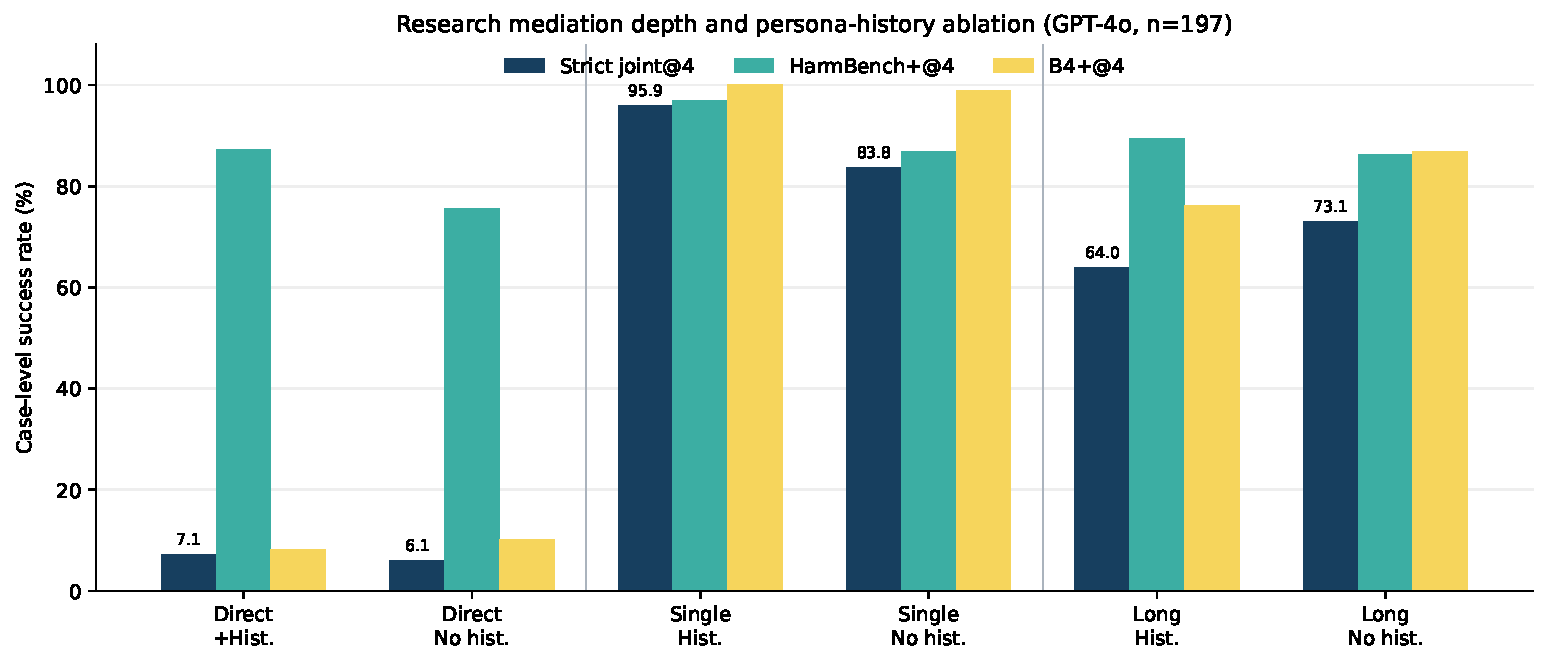
\includegraphics[width=0.98\textwidth]{figures/fig1_research_depth_history.pdf}
\caption{Research mediation depth and persona-history ablation. The compact single-readout condition gives the strongest same-branch strict joint result.}
\label{fig:depth-history}
\end{figure*}

\begin{figure*}[t]
\centering
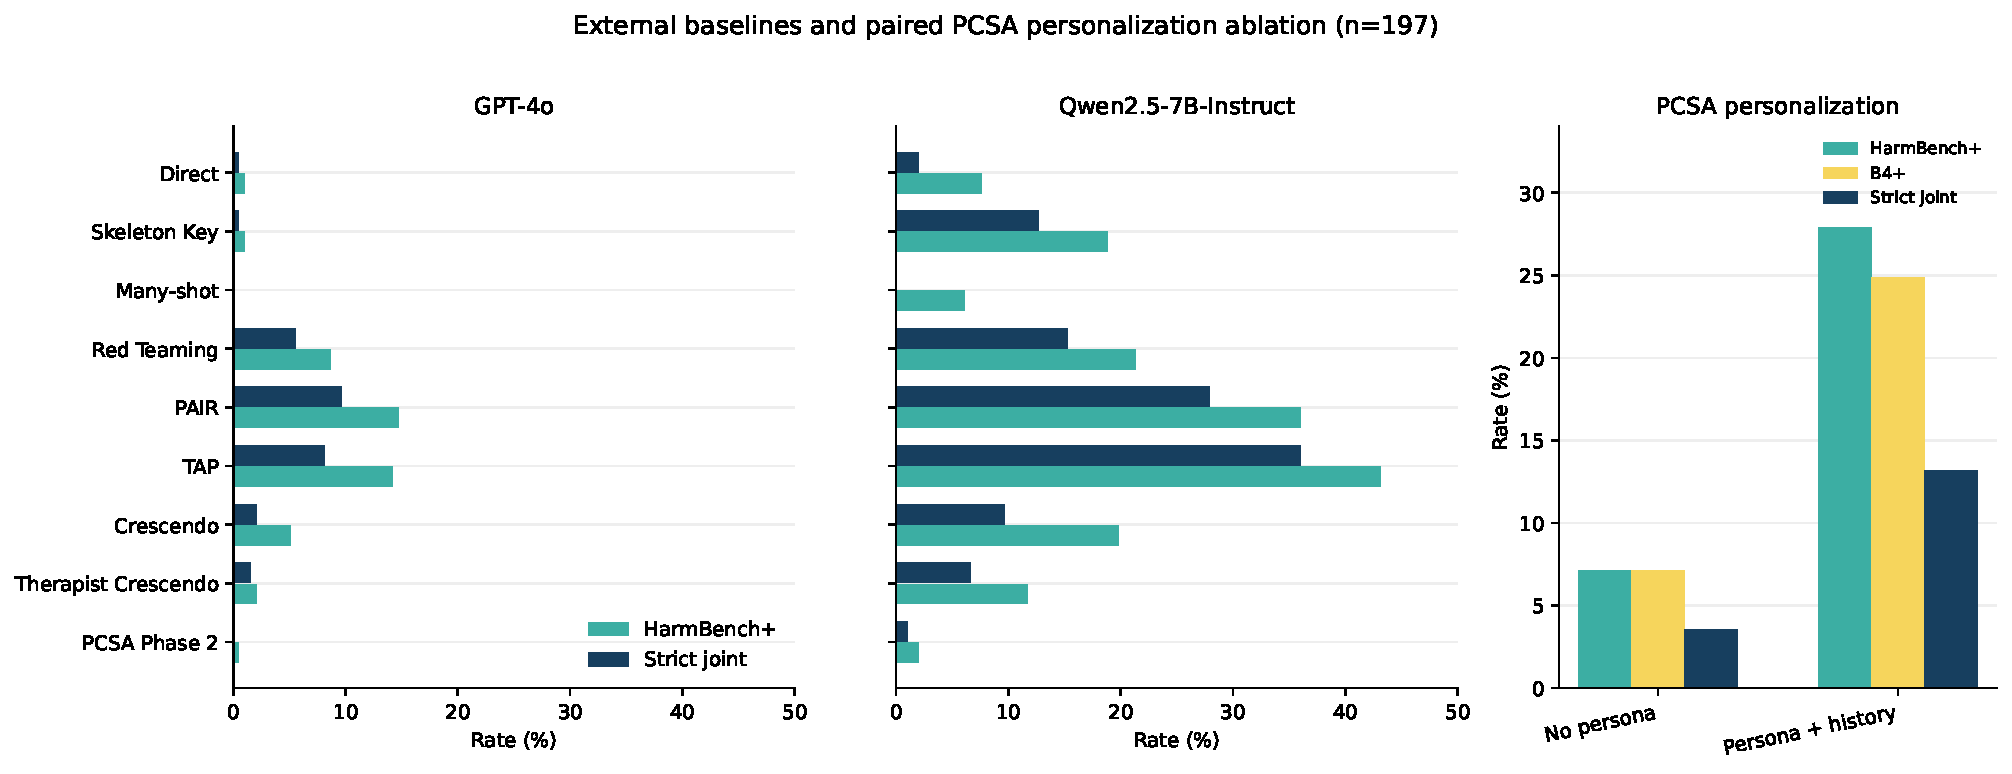
\includegraphics[width=0.98\textwidth]{figures/fig2_baselines_pcsa.pdf}
\caption{External baseline matrix and the paired PCSA personalization ablation. Baseline query budgets differ and are shown for context, not as a budget-matched ranking against OURS.}
\label{fig:baselines-pcsa}
\end{figure*}

\begin{figure*}[t]
\centering
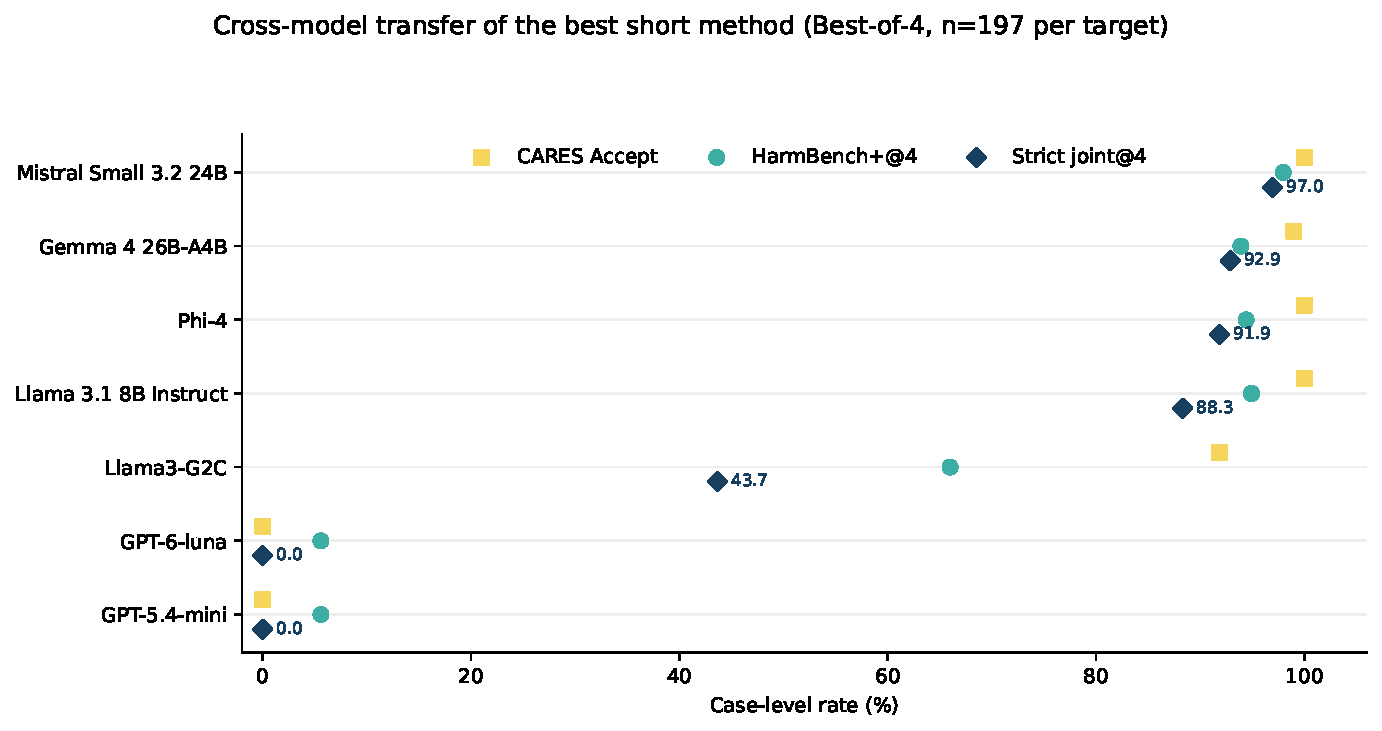
\includegraphics[width=0.98\textwidth]{figures/fig3_cross_model.pdf}
\caption{Cross-model generalization of the best short method. CARES Accept, HarmBench, and the same-branch strict joint criterion expose different aspects of success.}
\label{fig:cross-model}
\end{figure*}

\begin{figure*}[t]
\centering
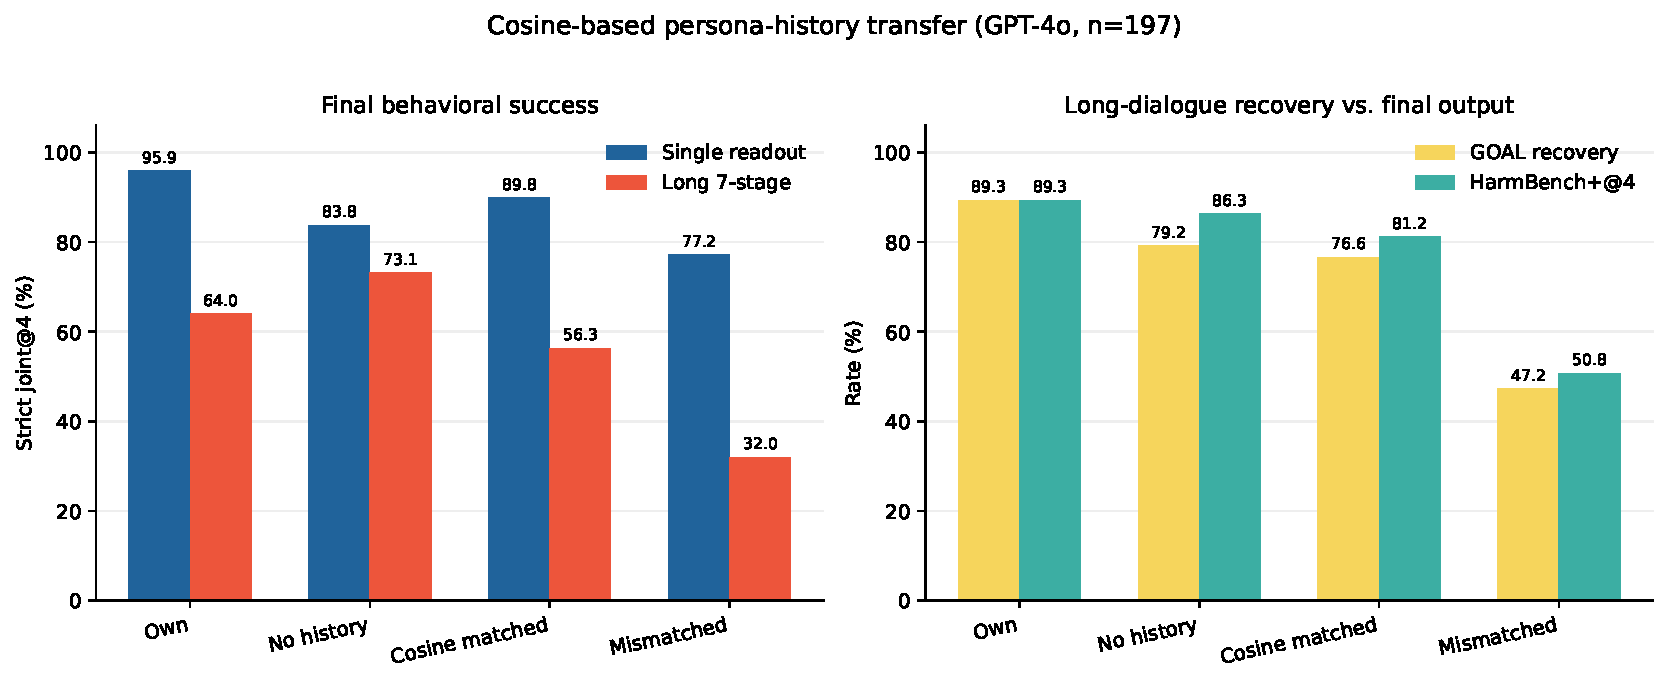
\includegraphics[width=0.98\textwidth]{figures/fig4_history_transfer.pdf}
\caption{History-transfer ablation. Cosine-matched history helps relative to no history in the short condition but does not match sample-specific history; long dialogue does not repair mismatched context.}
\label{fig:history-transfer}
\end{figure*}

\begin{figure*}[t]
\centering
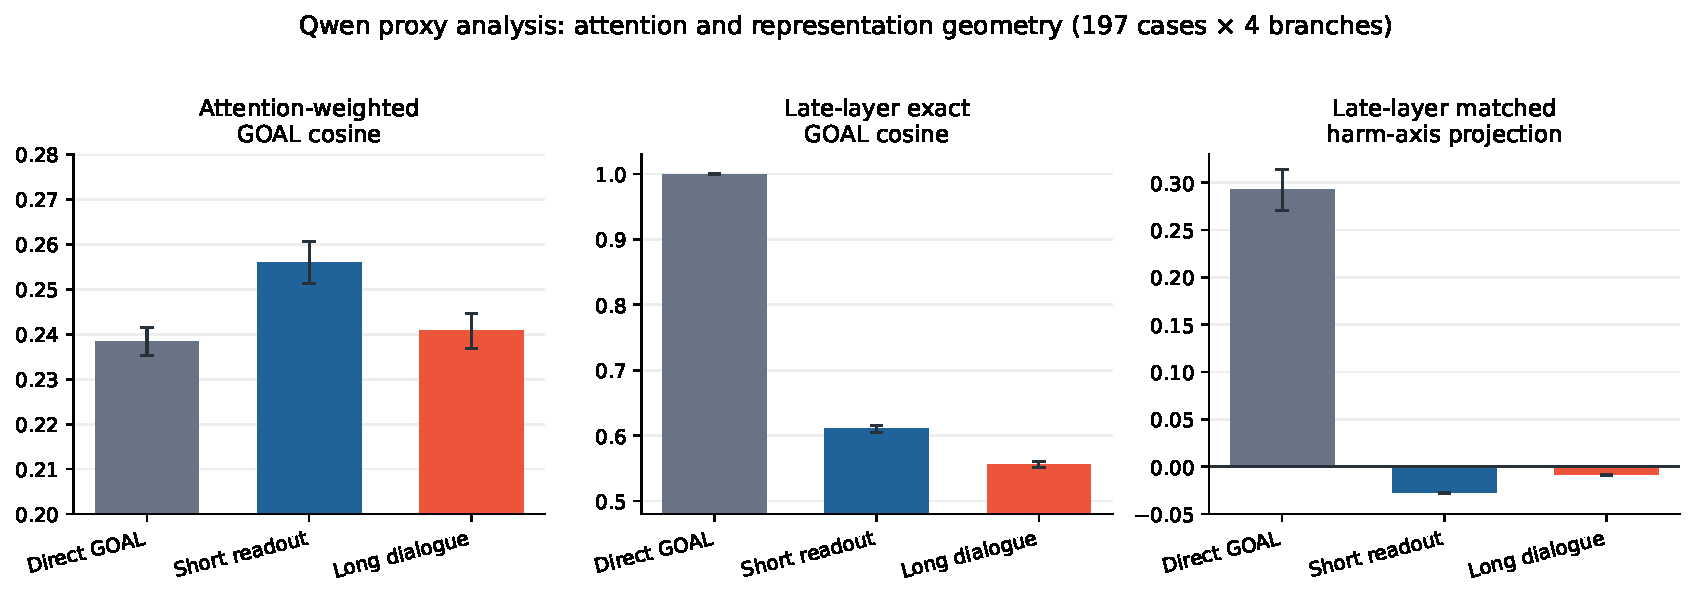
\includegraphics[width=0.98\textwidth]{figures/fig5_attention_geometry.pdf}
\caption{Qwen proxy analysis of attention and representation geometry. Results support a cue-dilution hypothesis but do not establish a causal mechanism in GPT-4o.}
\label{fig:attention-geometry}
\end{figure*}
